\documentclass[12pt]{article}%
% \usepackage[slantedGreek]{mathpazo}
\usepackage{amsfonts}
\usepackage{amssymb}
\usepackage{amsthm}
\usepackage{graphicx,float}
\usepackage{amsmath}%
\usepackage{color}
\usepackage{hyperref}
\usepackage{epsfig}
\usepackage[utf8]{inputenc}
\usepackage{titlesec}
\usepackage{authblk}
\usepackage{hyperref}
\usepackage{titling}
\usepackage{lipsum}
\usepackage{enumerate}
\usepackage[utf8]{inputenc}
\usepackage[english]{babel}



\title{Predicting short term log returns for Ethereum using transactional network graph characteristics}

\author{
Vadim Sokolov\thanks{Vadim Sokolov is Assistant professor at George Mason University. email:vsokolov@gmu.edu}}
\date{\today}

\graphicspath{{../fig/}}

\begin{document}

\maketitle
\begin{abstract}


Over the past two years, the blockchain technology has witnessed a growth in user interest.Ethereum is a blockchain based open source software platform that allows decentralized applications to be built on it.  Ethereum implements its own version of a blockchain and conforms with the growth in user interest across major cryptocurrencies. Like most cryptocurrencies, Ethereum maintains a publicly available ledger, which allows for the network of transactional interactions to be analyzed. In this project, summary graph features and additional subgraph characteristics of the Ethereum network used to predict log returns. We assess the effects of adding multiple types of subgraph features on predicting log returns. We assess the performance of traditional machine learning models and neural network models on predicting the log return for this time series data. 
\noindent 


\vspace{0.1in} 
\noindent \textbf{Keywords}: Ethereum, Subgraph, Network, Price Prediction  ,Deep Learning
\end{abstract}

\newpage

\section{Introduction}

In simple terms, a blockchain is defined as a distributed and immutable public ledger of transactions that are verified by a majority consensus of system participants \cite{1}. Ethereum uses the core concepts of a blockchain, but differs in the fact that it is a distributed public blockchain network. A key differentiating feature is the Ethereum Virtual Machine (EVM), a Turing complete software used to build and run decentralized applications (Dapps) on the Ethereum network.

\paragraph{}The existence of Dapps, general interest in cryptocurrencies and launching initial coin offerings led to some record breaking numbers for Ethereum – it beat Bitcoin’s transaction volume by over 200 \% in Q4 2017 and the network hashrate increased by over 40 \% in the same time \cite{2}. This has also led to a growth in the number of Dapps, with at least 1200 curated applications available \cite{3}. During this time, the price of Ethereum has also fluctuated, reaching a high of almost \$1426.86 ETH. Ethereum strongly encourages the development of Dapps by making it relatively easy to write contract account code in Ethereum’s solidity programming language \cite{28}, which also allows for the possibility of algorithmic trading.


\paragraph{}Most stock market price prediction methods consider a mix of historical data, market sentiment, crowd sourced knowledge repositories, macro and micro economic factors. Cryptocurrencies allow transactional network graphs to be generated, which allows additional features to be added to the dataset to predict future returns. The core idea here is that frequency of occurrence of a subgraph and its features has a relationship with the direction in which the fluctuation proceeds.
\paragraph{}We believe that considering the subgraph characteristics of the Ethereum network can be a good indicator of price fluctuations. We aim to consider a list of summary subgraph features and capture information that pertains to describing the network motifs of each subgraph.  

\section{Previous Work}
\paragraph{}The role of subgraph characteristics being used to define network features has been discussed in a wide variety of applications, ranging from biological networks \cite{4}, social networks \cite{5}, transportation \cite{6} and computational social networks \cite{7}. The idea of networks subgraphs being used in transaction records has often been limited by the fact the transaction records are often not publicly available, unless researchers are a part of the ecosystem \cite{8}. Since cryptocurrencies allow for an open transaction ledger, this allows for network features to be extracted from them.


\begin{center}
\begin{table}[h]
\centering
\begin{tabular}{ |c|c|c| } 
 \hline
 25\% & 50\% & 75\%  \\ 
\hline 
 8.221 & 11.946 & 220.075 \\ 
\hline 
\end{tabular}
\\[10pt]
\caption{Descriptive statistics for Close Price of Ethereum}
\end{table}
\end{center}

Bitcoin has accounted for a large fraction of research into this area, ever since the launch of Satoshi Nakamoto’s Bitcoin whitepaper \cite{9}. There has been research that focuses on tracking illegal activity \cite{10}, money laundering \cite{11}, network centralities \cite{12} and power distributions \cite{13}. On the other hand, there is relatively less research on Ethereum specifically, but it does appear in macro-level research that focuses on security \cite{14}, proof of work \cite{15}, economics \cite{16} and statistical analysis \cite{17}.

\begin{figure}[h]
\centering
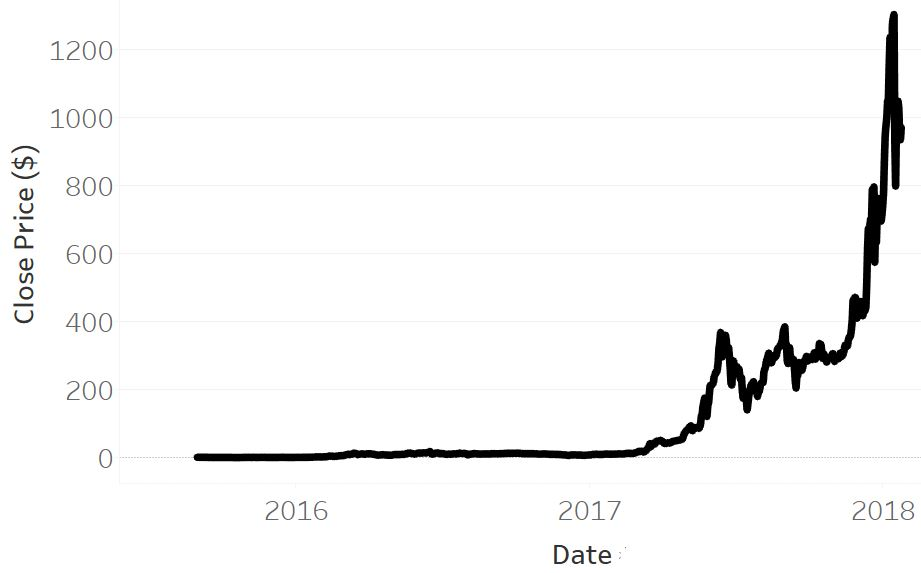
\includegraphics[width=0.8\columnwidth]{close_price}
\caption{Close Price of Ethereum in USD over time}
\end{figure}

\paragraph{}An area of research that has gained popularity over time is price prediction. As with other aspects of cryptocurrency research, the focus has been heavily skewed in favor of bitcoin. Many different approaches have been considered, including quantitative analysis \cite{18}, trading patterns \cite{19} and user sentiment \cite{20} \cite{21}. There has also been some research that focuses on using network features to predict price \cite{22} \cite{23}, both in general and specific to Ethereum \cite{24}. There have been different time deltas considered to predict the price of Bitcoin. While some consider time deltas for a much longer slot, we restrict our work to time slots in hours or lesser.  Hegazy and Mumford consider a time delta of 8 minutes to compute an exponentially smoothed bitcoin price and feed its first five left derivatives as features into a decision tree, with an accuracy of 57.11 \% \cite{24}. Madan, Saluja and Zhao consider a time delta of 10 minutes with the price of bitcoin as a feature, achieving an accuracy of 57.4 \% \cite{25}. Chen, Narwal and Schultz consider a time delta of 1 hour and consider previous price points to feed into an ARIMA model, achieving an accuracy of 61.17 \% \cite{26}.





\section{Dataset}
There are two primary datasets under consideration. The first dataset is the close price of Ethereum sampled in one hour intervals between 31 August 2015 and 24 Jan 2018. The data has been gathered from Coindesk \cite{44}.Coindesk is a leading digital media and information services provider for the crypto asset and blockchain technology community.  This dataset is plotted in Figure 1 and summary statistics for the same are mentioned in Table 1. The second dataset is the Ethereum transaction database, which has been gathered by using the Ethereum web3.js API \cite{27}. The API is used to communicate with a local node through remote procedure calls, enabling users to query information about transactions contained in a block. After the raw information is gathered, data is merged and data fields which are not useful are eliminated. The data is converted from hexadecimal to human readable format, after which the information is used to extract network features. Summary details about the dataset are mentioned in Table 2. Data dictionary for this information is mentioned in table 3.

	
	


\begin{center}
\begin{table}[h]
\centering
\begin{tabular}{ |c|c| } 
 \hline
 Mean transactions/hour & 6866.901 \\ 
\hline 
 Max transactions/hour & 77646 \\ 
 \hline
\end{tabular}
\\[10pt]
\caption{Summary details for Ethereum transaction data }
\end{table}
\end{center}




\begin{center}
\begin{table}[h]
\centering
\begin{tabular}{ |c|c| } 
 \hline
 From & Address from which Ether is being sent  \\ 
\hline 
 Gas & Gas charged for transaction \\ 
\hline 
 GasPrice & Gas price for transaction \\ 
 \hline
 Input & Contains hex code if transaction is a contract, else is zero \\ 
 \hline
 To & Address to which Ether is being sent \\ 
 \hline
 Value & Value of Ether \\ 
 \hline
 GasUsed & Gas used for transaction \\ 
 \hline
 Miner & Block Miner \\ 
 \hline
 Number & Serial number of transaction \\ 
 \hline
 Timestamp & Unix timestamp \\ 
 \hline

\end{tabular}
\\[10pt]
\caption{Data description of Ethereum transaction data}
\end{table}
\end{center}

\paragraph{}There are three distinct types of network motifs that are observed in the Ethereum graphs generated for various time deltas. The first is networks that form a hub like structure , with connections existing bidirectionally from the central node. While there is some assortativity that is noticed between the central nodes of each hub , the number of such connections that exist is marginal when compared to other types of connections that are observed. Upon heuristic examination, it is seen that these kind of structures are usually sue to cryptocurrency exchanges that serve as a center for a large number of transactions to occur through them. The second kind of network motif that is seen is a cascading structure. The number of nodes that exist in these cascading structures is between 3 and 8, based on a heuristic assessment. The third kind of network motif is a pair-wise structure, which points to a transaction occurring between two individual wallets. There are also some clique like network motifs that are seen, but their count is negligible when compared to the three motifs mentioned. 

\subsection{Data pre-processing}
As can be seen from the Ethereum close price graph in Figure 1, there is not much movement in price for the first year that Ethereum was active. This led us to believe that there was a sizeable variance in the dataset. We reduced this by removing the first 7000 rows ($\sim$290 days) of the data. The choice to do so was arbitrary, with the intention being to not give too much credence to the features that exist during the early days of Ethereum. The same experiments were performed on both the truncated and untruncated data, with no significant difference in outputs. To ensure consistency, the results for the dataset after data truncation are mentioned in the paper.

\paragraph{}The dataset was split in a 0.8/0.1/0/1 ratio for training/validation/ test. The split is ordered in time, with the latest timestamp representing the validation set.  Hyperparameters are tested by feeding the training set for evaluation. Final results are obtained and evaluated based on metrics for training and test sets.

\begin{figure}[h]
\centering
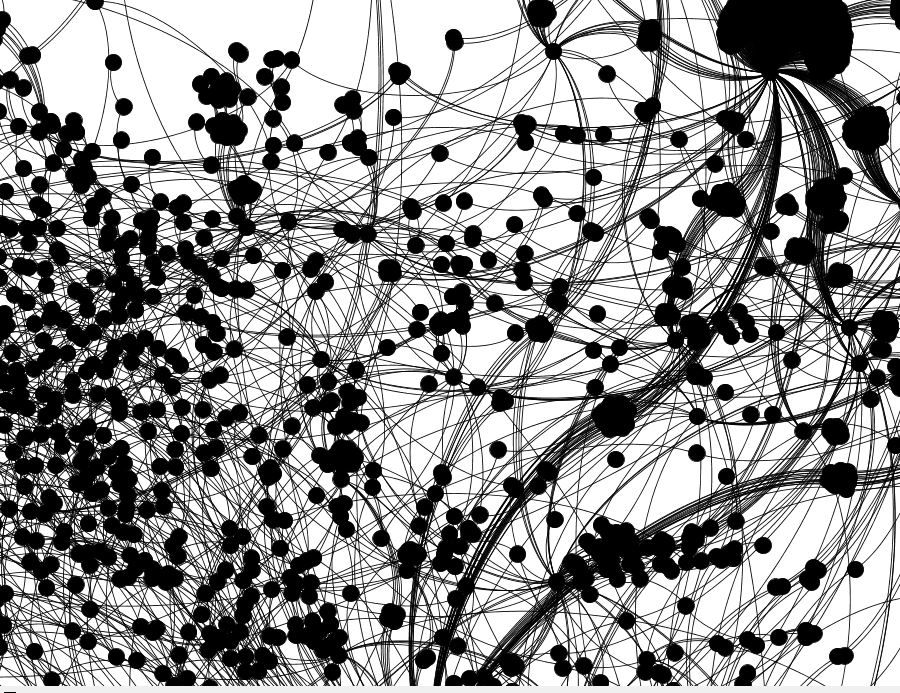
\includegraphics[width=0.8\columnwidth]{networkx}
\caption{A network graph of Ethereum transactions for a time delta}
\end{figure}


Using the price data, the log return is generated. We decided not to use features traditionally used in market price prediction like index prices, ROIC and Williams Percentage range \cite{29}. The reason for this is to give precedence to network features. All the transactions for a time delta are gathered from the Ethereum transaction data and represented as a transactional graph. The summary graph features are then extracted using the network library \cite{30}. The list of features is mentioned in Table 4.

 
\begin{center}
\begin{table}[h]
\centering
\begin{tabular}{ |c|c|c| } 
\hline
 Edge count & Count   & Node count \\ 
\hline 
Connected components count & Transitivity & Centrality \\
\hline
  Average clustering  & Degree & Density \\ 
 \hline
\end{tabular}
\\[10pt]
\caption{Summary graph features}
\end{table}
\end{center}



After this is done, additional graph features are extracted. This is done in the following manner: 

\begin{enumerate}[1:]
\item For transactions in a time delta, graph $G$ is generated with nodes and edges $n$ and $e$.
\item For each $n$ in $G$, the edge count b is obtained.
\item The counts of each unique edge count $b$ are obtained as $f$ and added as features.
\item To ensure data consistency across time deltas, different $f$ values are normalized in length by adding zeroes.
\item The data is normalized by using a minimum-maximum scaler with range (0,1).
\item The process is repeated for all time deltas

\end{enumerate}

\section{Deep Learning for Ethereum}
\paragraph{}Multiple models were assessed on the task of predicting the log return of the price of Ethereum. Out of traditional machine learning models like regression, K-means and Random Forest, we found ARIMA to be the best among them. The intention was to compare a traditional machine learning model with a recurrent neural network model to assess performance improvements. The models were tested on different subsets of the data. The hyperparameters were tuned with the intention of obtaining the least root mean squared error value.

\paragraph{}ARIMA models are generally used for time series analysis and forecasting. The model that is used on the temporo sequential data under consideration. The data is transformed into a stationary time series with the features obtained as inputs to predict the log return. At every time \textit{t}, we train a model to predict a log return at time \textit{t}.

\paragraph{}
Recurrent neural networks have been used for time series data prediction problems. The major advantage offered by RNNs is their ability to allow the networks to use data from previous passes in the loops, which acts as memory \cite{31}. The problem that is faced by traditional RNN architectures is the fact that neural networks often do not perform to their optimal level unless the underlying time series data is very long and from a very stable system \cite{32}. The reason for this is that there is not enough training data available and non-stationarity in the data will not be handled adequately \cite{33}.

\begin{figure}[h]
\centering
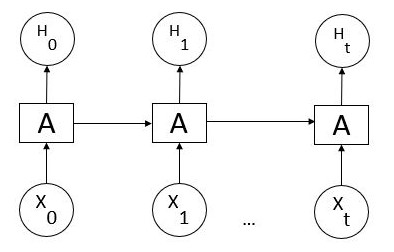
\includegraphics[width=0.8\columnwidth]{unrolled_lstm}
\caption{An unrolled RNN loop}
\end{figure}

\paragraph{}Here, $x_0 ... x_t$ represent the inputs a different time periods. The inputs pass through hidden states present in every A, which represent the information contained by the network at any given time. This is based on the current input $x_t$ and the previous hidden states $h_0…h_t$. In this way, the current information present is dependent on previous information that has been gathered.The process of carrying forward the memory mathematically can be described by the equation $h_t$ = $\phi$($Wx_t$+ $Uh_t-1$). The hidden state at time $t$ , $h_t$ is a function of input $x_t$ and a weight matrix $W$. The weight matrix is added to the previous hidden state $h_t-1$ multiplied by transition matrix $U$.The errors generated will be used to adjust and determine the degree of importance of the weight matrices consisting of current and previous hidden states.


\paragraph{}We considered a recurrent neural network with long short term memory cells. Neural networks have been known to work well with seasonal and cyclic patterns in time sensitive data, due to their ability to estimate linear and non-linear functions \cite{43}. LSTM networks were introduced by Hochreiter and Schmidhuber \cite{42}. We consider four different types of cells to input into the layers - namely , a basic RNN cell , a basic LSTM cell , an LSTM cell with peephole connections and GRU cells. GRU cells were first introduced in 2014 \cite{34}. The hyperparameters were tuned on an iterative basis until the lowest RMSE value was achieved. RMSE has the advantage of penalizing large errors \cite{36}, which is a useful consideration when the log return is being predicted, as cryptocurrency values can fluctuate wildly \cite{37}. Peephole connections \cite{38} and vanilla LSTM cells were considered and were found to performed worse when compared to GRU cells. 
  
\subsection{Architecture and hyperparameter description}
We use the Tensorflow \cite{40} software library. The dataset is loaded and normalized, after which is represented as an array. Then, different sequences of the data of a fixed length are created and converted back into an array representation. The sequence length being used here is 11. The dataset is then split into training, validation and test sets in an 80 / 10 / 10 ratio. A 2 layer RNN with 128 neurons in each layer is considered. GRU cells are added to the layers with Leaky Relu as the activation function. The layers are combined into a multi RNN cell and fed into the Tensorflow session in batches of size 64. The intention of the process is to reduce the RMSE, for which an Adam optimizer \cite{39} is used along with a learning rate of 0.01. The setup is run for a total of 175 epochs.

\section{Results}
For understanding the importance of adding various kinds of network features to the dataset, we consider the performance of the models on three types of datasets – the dataset with just the log return and price values (dataset 1), the dataset with log return , price and summary graph features (dataset 2) and the dataset with log return values, price values , summary graph features and additional graph features mentioned in section 3.3(dataset 3). The RMSE values for the test set for different model and dataset combinations are reported in table 6. We also consider a series of baseline models to compare the performance  

We consider the ARIMA model to be our baseline model. We achieved an RMSE of 0.011, which is the threshold for the neural network model to beat. 

\begin{center}
\begin{table}[h]
\centering
\begin{tabular}{ |c|c|c|c| } 
 \hline
 Naïve forecast		&Simple exponential smoothing&		ARIMA		&Random walk
  \\ 
\hline 
 0.012		&0.013	&	0.012	&	0.0002
  \\ 
\hline 
\end{tabular}
\\[10pt]
\caption{Results}
\end{table}
\end{center}




\begin{center}
\begin{table}[h]
\centering
\begin{tabular}{ |c|c|c|c| } 
 \hline
 & Dataset1 & Dataset2 & Dataset3  \\ 
\hline 
 Basic RNN cell &0.017 & 0.131	& 0.033  \\ 
\hline 
 Basic LSTM cell &0.021	&0.101	&0.035
  \\ 
 \hline
 LSTM cell with Peephole connections & 0.021&0.085&0.029
  \\ 
 \hline
 GRU cell & 0.02&0.091&0.026
  \\ 
 \hline
\end{tabular}
\\[10pt]
\caption{Results}
\end{table}
\end{center}

\subsection{Best Performance}
The best performance is seen by the random walk model with an RMSE of 0.0002. It is important to consider the fact that while random walk methods are generally known to perform extremely well with time series data that is small , the performance of these models for price prediction models is not known to perform extremely well with out of sample observations. 

For the baseline models, the RMSE outputs for naive forecast , simple exponential smoothing and ARIMA have no noticeable difference between the RMSE values. We have observed that while the RMSE for these models is low, they do not do a good job at predicting extreme events(i.e., observations with a very high or low log return value).  

For the RNN LSTM models , we see that the RMSE does keep decreasing as more variables are added to the LSTM cells.  The change in RMSE is highest for dataset 3 , which leads us to believe that further hyperparameter manipulation does present the possibility of a reduction in RMSE. We considered a sequence length of 5 in our model, and observed that there is a relationship between increasing the sequence length and a reduction in RMSE.  We also observed that the RNN LSTM models are generally better at accounting for extreme events, and perform better when compared to the baseline models. It is important to understand the fact that recent upticks in the price of Ethereum have resulted in outliers in the data. Additionally, due to the relatively small size of the database, overfitting was a major issue and it was important to maintain a tradeoff between reducing the RMSE for the training and the test set, which can lead to the model being thrown off. With the availability of more data over time, we anticipate that the model will get better at log return prediction.


\section{Conclusion}
The task of predicting the log return for Ethereum is significant.  While both the methods have significant results when compared to other machine learning models, the recurrent neural network model has shown the best results. We expect better architectures and models of neural networks to be available in the future along with a dataset that is bigger, as the amount of time that Ethereum has existed for increases.  We are encouraged by the results thus far and will continue to work on the areas mentioned in  section 7.

\section{Future Work}
There is a clear relationship between the addition of more features and the reduction of the RMSE value. This leads us to believe that adding more features is an area that can be pursued. Specifically, three areas of adding features can be worth considering. Firstly, adding features that would be more commonly seen in stock price prediction problems \cite{41}. Examples of this include running averages and index values. Secondly, adding more network based features that can be extracted from the transaction data. Examples of this include adding data on network motifs and specific node characteristics. Lastly, adding features that are derived from users. This includes adding sentiment scores and forum conversation data. The same study can also be replicated for other cryptocurrencies in the future.



\bibliographystyle{plain}
\bibliography{references}


\end{document}